\documentclass[12pt, a4paper]{article}

\makeatletter
\begingroup\endlinechar=-1\relax
       \everyeof{\noexpand}%
       \edef\x{\endgroup\def\noexpand\homepath{%
         \@@input|"kpsewhich --var-value=HOME" }}\x
\makeatother

\def\overleafhome{/tmp}% change as appropriate
\usepackage{fontspec}
\ifx\homepath\overleafhome
\setmonofont{CONSOLA.TTF}[
BoldFont=CONSOLAB.ttf,
ItalicFont=CONSOLAI.ttf,
BoldItalicFont=CONSOLAZ.ttf
]
\else
\setmonofont{Consolas}
\fi

\usepackage[title]{appendix}
\usepackage[onehalfspacing]{setspace}
\usepackage{subfigure}
\parskip=1mm plus 1pt
\usepackage{indentfirst}
\usepackage{forest}
\usepackage[export]{adjustbox}
\usetikzlibrary{arrows.meta, %提供Stealth[]箭头类型
angles} %提供angle pic
	\forestset{
	tree angle/.style={
		% !表示开始相对引用。u是父节点,n是下一个兄弟节点。他们都是short-form step。
		% pic {angle}: draw a small picture of type angle.
		% angle是来自\usetikzlibrary{angles}。
		% The angle pic draws an angle between the two lines BA and BC, where A, B, and C are three coordinates.
		tikz={\path () coordinate (A) -- (!u) 
			coordinate (B) -- (!n) 
			coordinate (C) pic [draw, angle radius=#1] {angle};}
	},
	tree angle/.default=5mm
}

\usepackage[section]{placeins}

\usepackage{xcolor}
\usepackage{algorithm}
\usepackage{algorithmic}
\usepackage{makeidx}
\usepackage{hyperref}
\hypersetup{
unicode=true,          % non-Latin characters in Acrobat’s bookmarks
pdftitle={},    % title   
%pdfauthor={爱让一切都对了},     % author   
%pdfcreator={爱让一切都对了},
%pdfproducer={OpenOffice.org 3.3},
breaklinks=true,
colorlinks=true,       % false: boxed links; ture: colored links
linkcolor=blue,          % color of internal links   
citecolor=blue,        % color of links to bibliography  
filecolor=magenta,      % color of file links   
urlcolor=cyan,           % color of external links  
}
\usepackage{xcolor}

\usepackage{url}
\def\UrlBreaks{\do\A\do\B\do\C\do\D\do\E\do\F\do\G\do\H\do\I\do\J\do\K\do\L\do\M\do\N\do\O\do\P\do\Q\do\R\do\S\do\T\do\U\do\V\do\W\do\X\do\Y\do\Z\do\[\do\\\do\]\do\^\do\_\do\`\do\a\do\b\do\c\do\d\do\e\do\f\do\g\do\h\do\i\do\j\do\k\do\l\do\m\do\n\do\o\do\p\do\q\do\r\do\s\do\t\do\u\do\v\do\w\do\x\do\y\do\z\do\0\do\1\do\2\do\3\do\4\do\5\do\6\do\7\do\8\do\9\do\.\do\@\do\\\do\/\do\!\do\_\do\|\do\;\do\>\do\]\do\)\do\,\do\?\do\'\do+\do\=\do\#}

\usepackage{listings}
\lstset{
%  %行号
%  %numbers=left,
%  %背景框
%  %framexleftmargin=10mm,
%  %frame=none,
%  %背景色
%  %backgroundcolor=\color[rgb]{1,1,0.76},
%  %样式
  keywordstyle=\color{blue}\bfseries,
%  identifierstyle=\bf,
%  numberstyle=\color[RGB]{0,192,192}, %行号的样式
  commentstyle=\it\color[RGB]{0,96,96},
  stringstyle=\rmfamily\slshape\color[RGB]{128,0,0},
%  %显示空格
%  %showstringspaces=false,
  basicstyle=\ttfamily\footnotesize, %修正大写字母间距过小
  columns=flexible, %修正大写字母间距过小
  breaklines=true, %对过长的代码自动换行
%  escapechar=!,
%  morekeywords={BEGIN}
  upquote=true,
  language=python,
  tabsize=4
}


\newcommand{\code}[1]{\texttt{#1}}
\newcommand{\citeWeb}[3]{#1, \url{#2}, Retrieved #3.}
\title{CS 188 Security Evaluation on Team Random's Project}
\author{Weikeng Yang\\405346443 \and
Yingzhe Hu\\505366341 \and
Qiqi Gu\\604253019 \and
Dongyao Liang\\705313832 \and
Shuhua Zhan\\705190671}
\date{Team name: Random\\[2mm]February 28, 2020}

\usepackage[numbers]{natbib}
\setcitestyle{square}

\usepackage{graphicx}

\begin{document}

\maketitle

\tableofcontents
\newpage
\section{Summary}
This report evaluates our own project, Google Play Advanced Search. We have the application source code, and the application has been deployed to Google Cloud, accessible via \url{https://beta.gqqnbig.me/}. We will evaluate the security of the source code and the server deployment.



The project uses a number of external components, among which, Bootstrap 4.4.1 and vuejs 2.6.11 are fairly new. People may not have enough time to evaluate their security implications. Only the code that loads bootstrap has the \code{integrity} and \code{crossorigin} attributes. We suggest to add them to other \code{<script>} elements.\textsuperscript{\cite{html-standard-script}}



%Requirement: A brief summary of your findings, including the approach(es) you took and what you learned. This should be at a high level (e.g., "Working from the design document, we decided to perform code review using the following techniques, supplemented by the following kinds of testing") and should include some conclusion about the security of the system (e.g., "Our analysis showed that the mitigations used to address security concerns in our system were effective," or "Our analysis reveals fatal security flaws that could be remediated in the following ways," or a statement of similar nature).   For evaluation of the other team’s project, remember that your goal is not to criticize their efforts, but to determine whether they achieved sufficiently secure results and to suggest improvements if they did not. 

\section{Security Evaluation Plan}

%Requirement: A description of your plan for the security evaluation, including steps to be taken, tools or approaches used, work assignments, and a schedule. Since it is likely that your plan required some adjustments, you should discuss the degree to which you followed your plan versus deviating from it, as well as explanations for such deviations.  

As the instructor mentioned in the lecture, we are going to evaluate our project security according to the following steps.

\begin{itemize}
    \item Security Design Review (02/21/2020)
    \item External Components Review (02/21/2020)
    \item Code Review (02/22/2020 - 02/23/2020)
    \item Tool Testing (02/24/2020 - 02/26/2020)
    \item Data Security, DDOS attack, and SSL Test (02/27/2020) 
\end{itemize}
    
Testing is one important element of our evaluation. We plan to use these testing tools to evaluate our project:
\begin{itemize}
    \item Network sniffers
    \item \code{Nmap} as Port scanners 
    \item \code{OWASP ZAP} for Web security testing
%    \item Tools to test crypto usage
    \item Fuzz testing tools
%    \item Password crackers
    \item Database security scanners
%    \item Mobile app security testers (MASTs)
    \item Interactive application security testing (IAST)
    \item SSL Test using online tool immuniweb
    
\end{itemize}


As mentioned, we will evaluate two parts of project Google Play Advanced Search, checking the security issues in the source code, and finding if the server on \url{https://beta.gqqnbig.me/} is properly protected.

When we were developing the project, we were already performing code review, ie. a team member creates pull requests (PR) for his/her changes, and an experienced team member will review the commits in the pull requests, approve the PR or request revisions. However, it is mainly Qiqi and Dongyao who review pull requests. We will ask other team members to read the code in hope that they find out something the PR reviewer missed before.

When we are doing security evaluation code review, candidate point strategies.

We will also check the security vulnerabilities of the dependencies of the project.

%Our plan for the security evaluation as follow:


\section{Security Evaluation Results}

Requirement: You should describe the results of your security evaluation, providing sufficient details to justify any conclusions you reach. This section should be significantly more extensive than the summary, containing a great deal more detail. If, for example, you found a dangerous race condition in the code, you should describe how you found it, what the security implications are, and suggest approaches for fixing it or ensuring that it is not exploited. 

\subsection{Security Design Review}
\begin{figure}[ht]
\centering
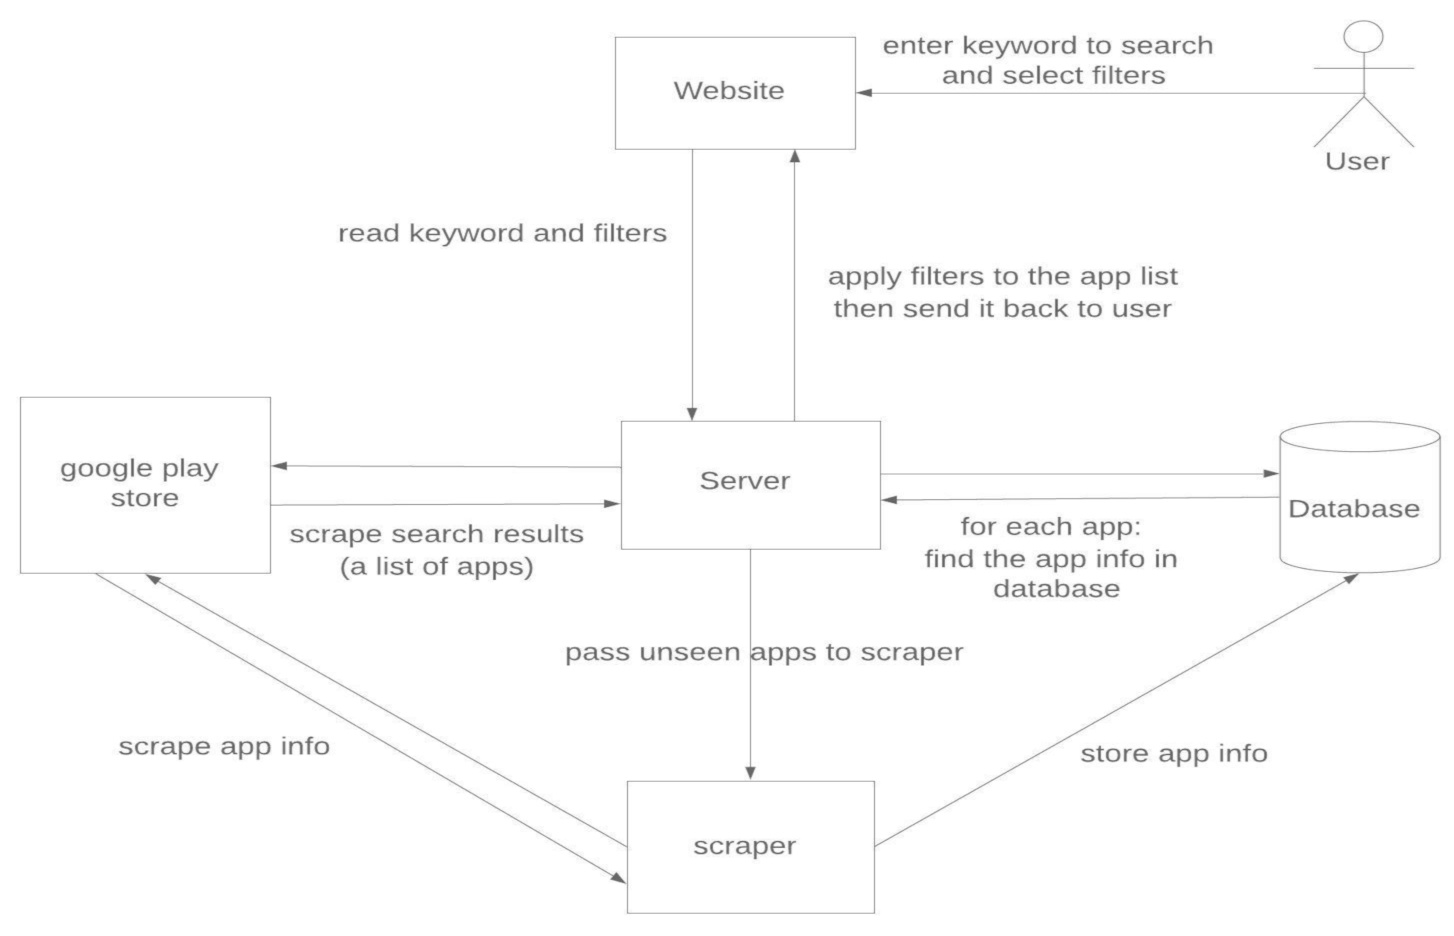
\includegraphics[width=0.8\textwidth]{Context_Diagram.jpeg}
\caption{Design Diagram}
\label{fig:design_diagram}
\end{figure}

Figure \ref{fig:design_diagram} is the design diagram extracted from the design document. We evaluate the design again. By looking at the source code at a high level, we conclude the implemented project largely matches the design, with a few exceptions.

\begin{figure}[ht]
\centering
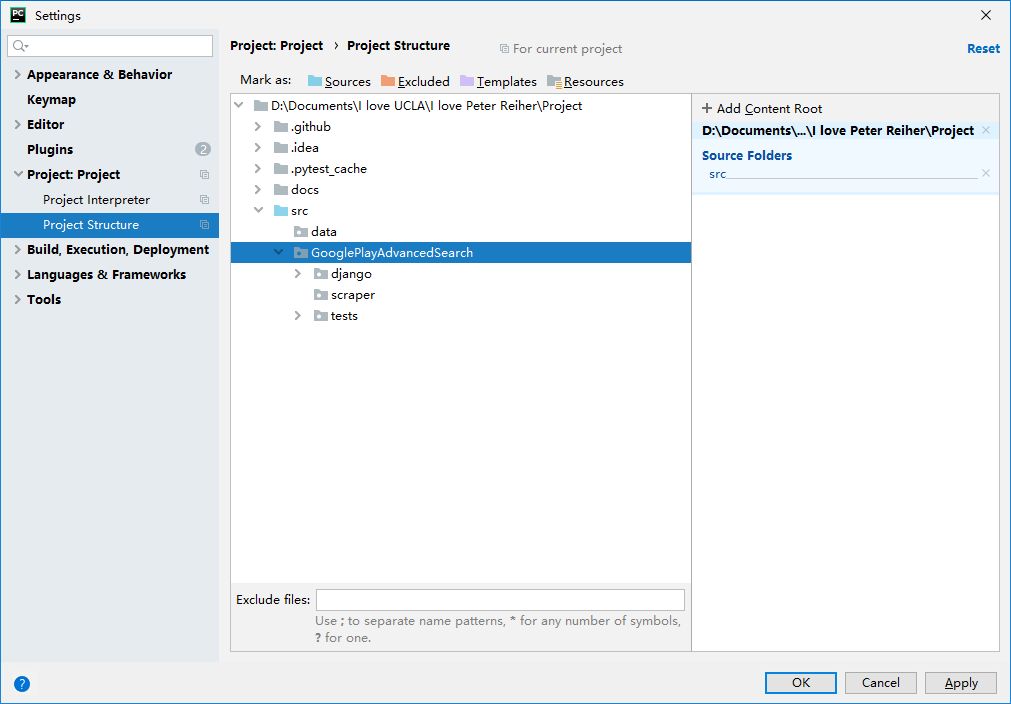
\includegraphics[width=\textwidth]{project-structure.png}
\caption{Project structure. \code{src} is the source code root.}
\label{fig:project-structure}
\end{figure}

The implemented project has 3 modules, well organized into a hierarchical namespace, see Figure \ref{fig:project-structure}. \code{src} is the source code root. tests is the additional module but since it's for automated tests, the addition is not a big deal.

The design diagram indicates there is a server component, but actually the django module and the scraper module both run on a server; the SQLite database is on the same server as well. Some functions, for instance \code{src/GooglePlayAdvancedSearch/DBUtils.py} are shared across modules. 

Unlike the design diagram, the implemented website talks to database, and run scraper as a standalone process. Both are found in \linebreak[4]
\code{GooglePlayAdvancedSearch\linebreak[0].django.web.Api}\footnote{All code are in namespace \code{GooglePlayAdvancedSearch}. Moveing forward, we will remove this prefix for conciseness and only say \code{django.web.Api}.}.

Moreover, the django module has some scraping abilities. It scrapes Google Play search result page, and if the module requires more information, it then calls scraper.

By looking at the design, we hold the threats to the application are: 1) Attackers attacking through the website; 2) Attackers attacking the server; 3) Malicious data injected from Google Play. There are also threats to end users: 4) Attackers may perform man-in-the-middle attack. 5) We have to prevent cross-site attack, and 6) check client side security vulnerabilities, mainly JavaScript.

We assign high priority to 1), 5); medium to 4), 6), low to 2), 3).

\begin{figure}[ht]
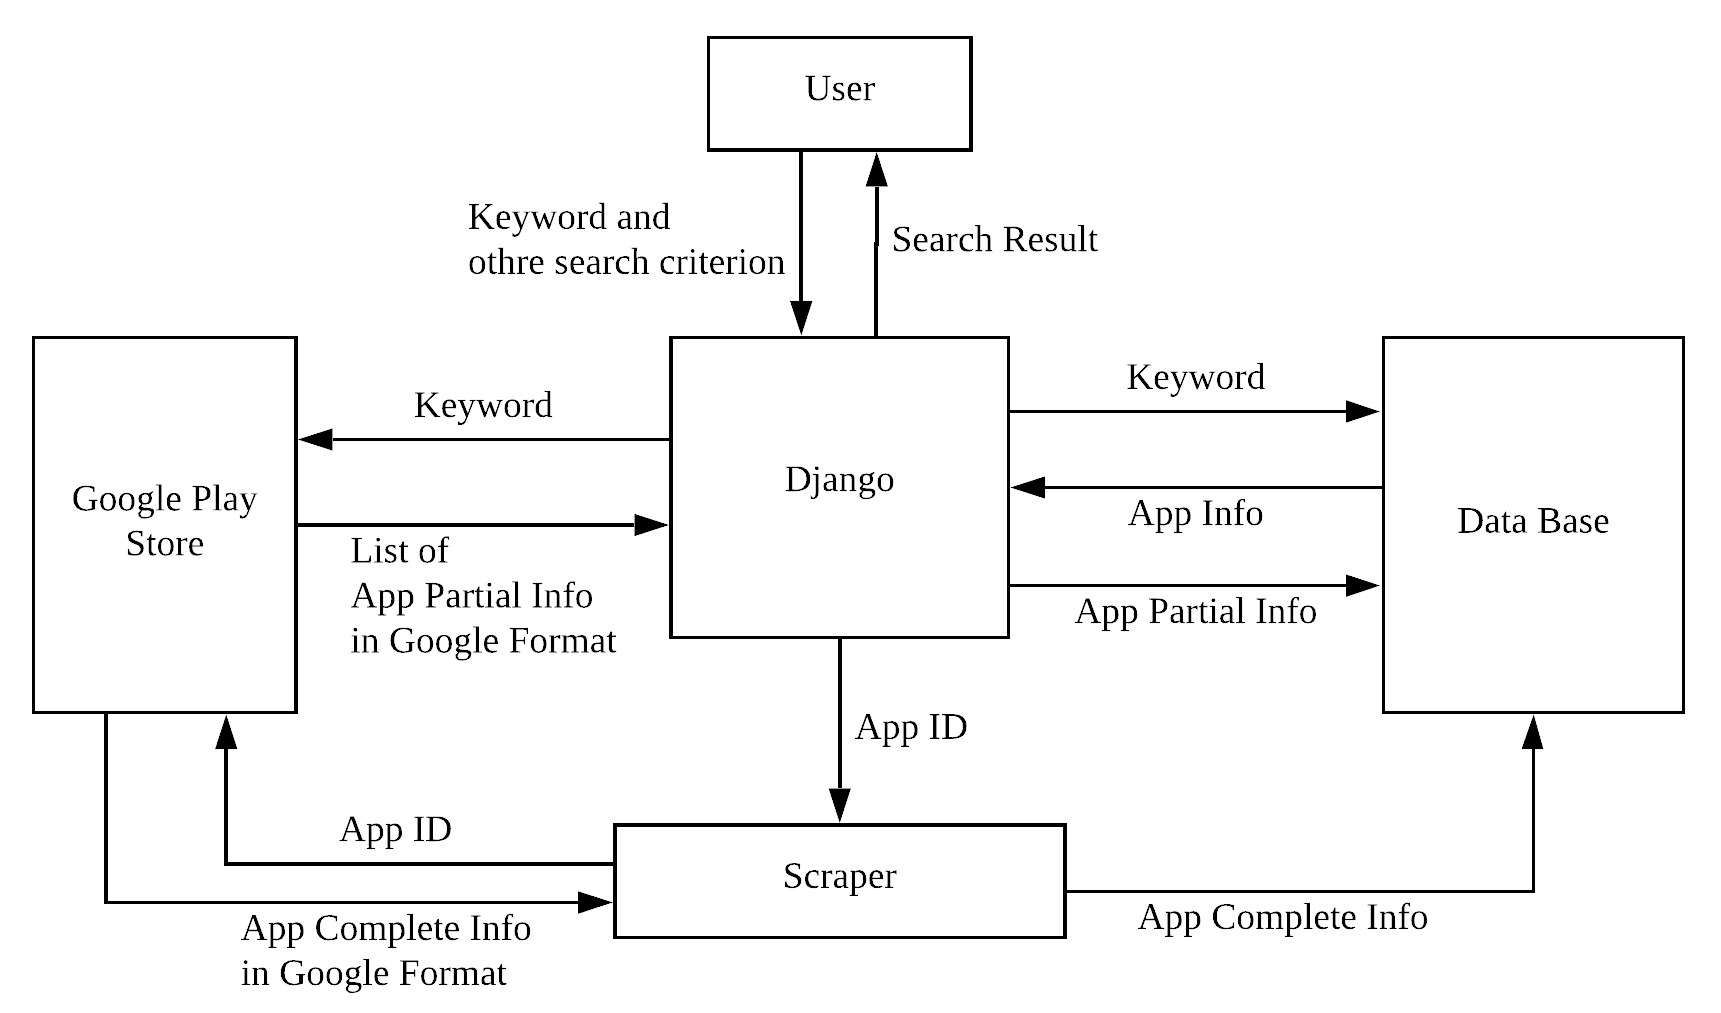
\includegraphics[width=\textwidth]{dataFlow.png}
\caption{Data Flow Diagram}
\label{fig:dataFlow}
\end{figure}

%Additionally, we also reviewed the data flow in the application, see Figure \ref{fig:dataFlow}. When an user searches our website (Google Play Advanced Search) for some specific apps, the keyword and other search criterion the user specifies enter the Django module. 1) Django sends the keyword to database and get a list of matching apps. The app info may be complete or partial. (Partial means the permission and category info are missing) Then Django filters the result based on the filter the user selected. 2) If the filtered result is less than 200, Django sends the keyword to Google Play Store, asking for potentially more results. Google search page returns app partial info encoded in JavaScript format. 3) Django saves the app partial info to database. 4) If our database now have all the information of apps the user needs, Django just returns the results to the user directly. 5) Otherwise, Django will record the missing apps ID and pass them to Scraper. 6) Scraper goes to Google Play Store to get complete information of the missing apps and save all the new data in database. 7) Finally, Django grabs all the complete information from database and returns them to user.

Additionally, we also reviewed the data flow in the application, and created Figure \ref{fig:dataFlow} showing the data flow.

\begin{enumerate}
    \item When an user searches on Google Play Advanced Search, the keyword and other search criterion the he specified enter the Django module. 
    \item  Django sends the keyword to database and get a list of matching apps. The app info may be complete or partial. (Partial means the permission and category info are missing) Then Django filters the result based on the filters the user selected.
    \item If the filtered result is less than 200, Django sends the keyword to Google Play Store, asking for potentially more results. Google search page returns app partial info encoded in JavaScript format. Django decodes them, and saves them to database.
    \item If our database now have all the information of apps the user needs, Django just returns the results to the user directly. 
    \item Otherwise, Django will record the missing apps ID and pass them to Scraper.
    \item Scraper goes to Google Play Store to get complete information of the missing apps and save all the new data in database.
    \item Finally, Django grabs all the complete information from database and returns them to user.
\end{enumerate}

Based on the process of data flow, we found that the most likely security issues - trace malicious input. In the original plan, we decide to use fuzz testing tools to evaluate our project, but we don't have enough time to go through it. We use python to create a script to search some very long and strange inputs on our website, see Figure \ref{fig:fuzz-test2}. The result shows that the website can detect it and output some error messages as feedback, see Figure \ref{fig:fuzz-test1}. 

\begin{figure}[ht]
\centering
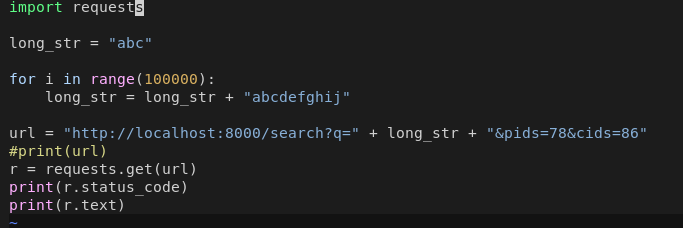
\includegraphics[width=\textwidth]{fuzz-test2.png}
\caption{Create a script search some long inputs on our website}
\label{fig:fuzz-test2}
\end{figure}

\begin{figure}[ht]
\centering
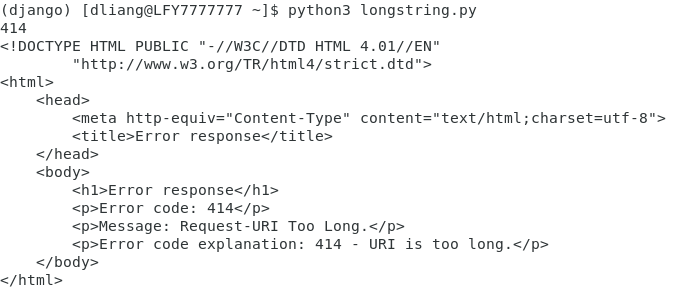
\includegraphics[width=\textwidth]{fuzz-test1.png}
\caption{Error message of long input}
\label{fig:fuzz-test1}
\end{figure}


\code{requirements.txt} lists the Python packages not developed by us. Besides, we use SQLite database and some client-side JavaScript libraries. Section \ref{dependency-evaluation} evaluates the security of these dependencies.


\subsection{External Components Review}
\label{dependency-evaluation}
\subsubsection{Python}
Python is a high-level programming language with a garbage collector for memory management. Python doesn't have buffer overflow issues, and doesn't have pointers. Therefore, we will not analyze buffer overflow for this project.

The design document states the application is written in Python 3.7, but neither \code{README.md} nor the shebang of the executables, eg. in \code{src/\linebreak[0]GooglePlayAdvancedSearch/scraper/Program.py}, specifies it very clearly. The problem is that another version of Python, which we may not test our project with thoughtfully, might run the code, and have some unexpected interactions with our code, producing bugs or security issues. The better way is to write \code{\#!/usr/bin/env python3.7} instead of \code{\#!/usr/bin/env python3}.

As of the shebang itself, it uses \code{/usr/bin/env}, which is supposed to pick the appropriate program to run the script. Using \code{/usr/bin/env} in shebang makes the script more portable, but attackers may inject their programs to \code{/usr/bin/env} and our project becomes the launcher of attackers' program.

\cite{python37-vulnerability} shows 23 vulnerabilities fixed in patches in Python 3.7, and 2 vulnerabilities unfixed. We found a few issues are clearly relevant to us. In CVE-2020-8315, at Python startup, an attacker's DLL might be loaded on Windows 7. Windows 7 is out of extended support on January 14, 2020.\textsuperscript{\cite{windows7}} Hence, we suggest Google Play Advanced Search to drop support on Windows 7. \cite{bpo-30730} is about Environment variables injection in subprocess on Windows. We use subprocess in the tests module, but we don't pass environment variables. The project might be susceptible to bpo-30458\textsuperscript{\cite{bpo-30458}} because the underlying packages use \code{urllib.urlopen(url)}. However, the URL passed into the function are from Google Play. The URL is unlikely to have a malicious form.

\cite{python37-vulnerability} is not a complete list, though. We also checked other sources. CVE-2019-9636\textsuperscript{\cite{CVE-2019-9636}} warns Improper Handling of Unicode Encoding in \code{urllib\linebreak[0].parse\linebreak[0].urlparse}, which is the function we are using. In \code{Api.search()}, an attacker may give us a crafted URL and cause an SSLError. The code catches the exception, and run \code{urlparse(e.request.url)}, where the vulnerability may be exploited.

Other Python 3.7 vulnerabilities are not immediately relevant to our project because we are not using the affected functions. We should check if the dependencies are using them, but due to time constraint, we didn't do.

\subsubsection{Python Packages}
Project Google Play Advanced Search includes a continuous integration workflow script, located in \code{.github/workflows/pythonapp.yml}. The workflow runs on GitHub Action servers, installs dependencies of the project by reading \code{requirements.txt}, and run automated tests. Since the workflow passes, we are pretty sure that \code{requirements.txt} lists every Python packages the application requires. Next, we will check security issues on the Python packages.

\url{https://app.snyk.io} automatically discovers security vulnerabilities on our project. Figure \ref{fig:snyk} shows the security report. SNYK finds only one high severity issue and one medium severity issue. 

\begin{figure}[ht]
\centering
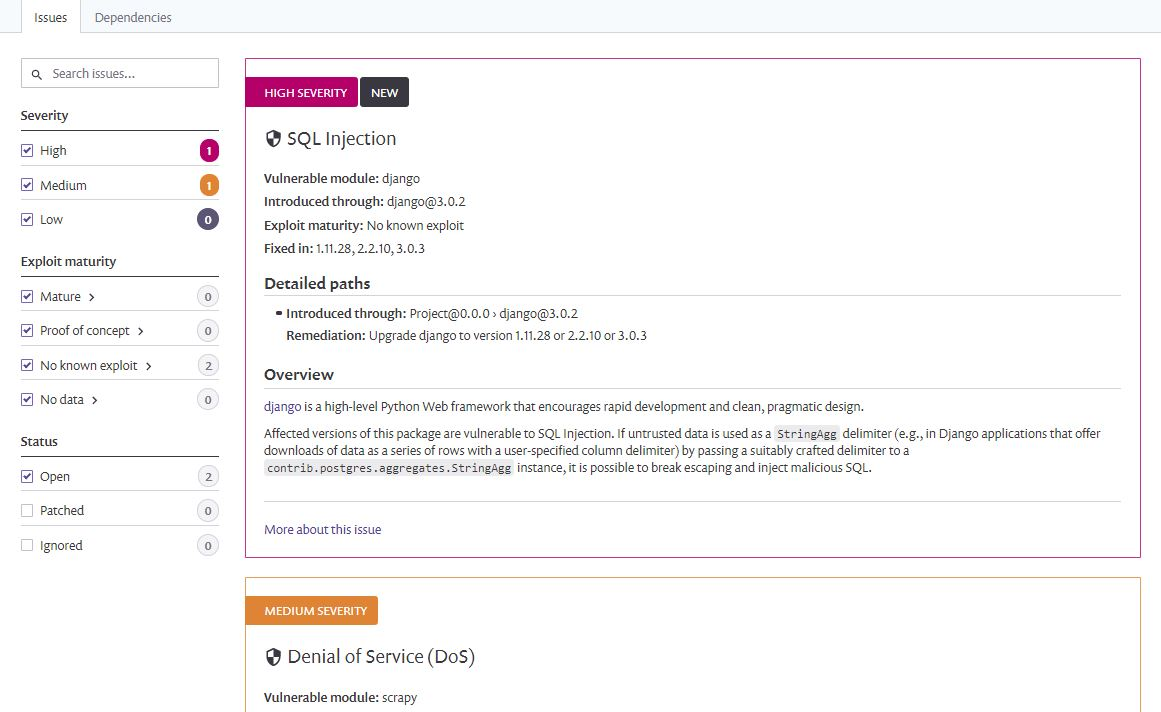
\includegraphics[width=\textwidth]{snyk.JPG}
\caption{The screenshot of SNYK analysis. We only have one high severity issue and one medium severity issue.}
\label{fig:snyk}
\end{figure}

According to the report, \code{StringAgg(delimiter)} is subject to SQL injection, but our code is not using this function. Other packages used by us don't depend on Django 3.0.2. Therefore we believe we are not susceptible to this issue.

The second Denial of Service vulnerability from Scrapy is irrelevant as well. According to the Scrapy issue\textsuperscript{\cite{scrapy-s3}}, DOS happens when communicating to Amazon S3 server. Since the scraper of Google Play Advanced Search stores scraped data to local database, we are invulnerable to this issue.

To increase confidence, we then manually go over the dependencies.

beautifulsoup4 is listed in \code{requirements.txt}, but we find the project is not using it. People are likely to install the application by running \code{pip install -r requirements.txt}. Thus an unnecessary component is installed to the machine. Although we didn't find major issues of beautifulsoup4 by searching the Internet, installing an unnecessary component brings some security risks anyway.


\cite{django-security-issues} lists other security issues in Django. CVE-2019-19844 is about Potential account hijack via password reset form. Our website doesn't have accounts, so we are immune to this attack. CVE-2019-19118 is about Privilege escalation in the Django admin. However, Google Play Advanced Search doesn't use Django admin site.

pyjson5\textsuperscript{\cite{pyjson5}} doesn't have a dedicated security issues page, but we searched the Internet and didn't find any security issues. However, we notice the project doesn't use this dependency, instead, some Python files import json, which is different than pyjson5. The same as beautifulsoup4, we believe installing an unnecessary component brings some security risks.

CVE-2019-18874 is a Double Free issue in psutil that Google Play Advanced Search uses. Double Free is that a program frees the same memory twice, that may lead to memory leak or alter the execution flow.\textsuperscript{\cite{double-free}} Although the bug was fixed in psutil 5.6.7, because \code{requirements.txt} doesn't specify the version of psutil, the project is vulnerable to this issue. But luckily, psutil is only used in the tests module, only developers or testers might be affected.

\cite{requests-security-vulnerabilities} discloses vulnerabilities in Python package requests. There are no known issues in requests 2.22.0.

The project uses Scrapy 1.8.0. Besides the issue mentioned in Figure \ref{fig:snyk}, Scrapy also had XML External Entity flaw.\textsuperscript{\cite{scrapy-xml}} Nevertheless, Scrapy 1.8.0 doesn't have other known security issues.

Twisted is a package required by Scrapy. In spite of that fact that Twisted had some security issues, for instance Man-in-the-Middle vulnerability and Improper Input Validation\textsuperscript{\cite{cve-twisted}, \cite{snyk-twisted}}, Twisted 19.10.0 that Google Play Advanced Search uses doesn't have known security issues.

urllib3 1.24.3 doesn't have known vulnerabilities although \url{https://www.cvedetails.com} and \url{https://snyk.io} shows some in its earlier versions, including Improper Certificate Validation (fixed in 1.24.2) and CRLF injection (fixed in 1.24.3). Again, the source code of Google Play Advanced Search didn't actually import the package.

Finally, the project requires pytest for automated testing. \code{requirements.\linebreak[0]txt} doesn't specify its version either, which is not a good practice. pytest doesn't have known security issues.


To confirm the project doesn't really need beautifulsoup4, json5, and urllib3, we removed them from \code{requirements.\linebreak[0]txt} and trigger continuous integration. We find urllib3 is a dependency of Twisted, but the other two are not needed. It's good to let Twisted determine the version of urllib3 because the author of Twisted can choose a vulnerability-free version.


\subsubsection{SQLite}
Google Play Advanced Search stories data in SQLite database. According to the README, the required version is 3.24 or higher. Version 3.24 was released on 2020-06-04, and it has 4 vulnerabilities.

CVE-2019-16168 may crash an application because of a sqlite\_stat1 sz field. The sqlite\_stat1 table is created by the ANALYZE command. However, Google Play Advanced Search doesn't use the ANALYZE command.

CVE-2019-8457 allows attackers to modify some system files but the attacker can't control which files are modified. Nevertheless, it's better to use a higher version of SQLite.

CVE-2018-20506 can run arbitrary SQL statements. This vulnerability is exploitable only if the application uses virtual table. Since Google Play Advanced Search doesn't use virtual table, it's not affected by this issue.

CVE-2018-20346 is a similar issue to CVE-2018-20506. Since Google Play Advanced Search doesn't use virtual table, it's immune to CVE-2018-20346 as well.

\subsubsection{Front-end Libraries}
The django component (the website) uses jquery, bootstrap, vuejs, and lodash for front-end rendering and interaction.

The website loads jquery 3.4.1, released on 2019-05-01, via content delivery network. \cite{jquery-341} claims there are no vulnerabilities in version 3.4.1, in spite that \url{https://www.cvedetails.com} has no data for this version.


The CSS part of bootstrap 4.4.1, released on 2019-11-28, is used by this project by the code in Listing \ref{lst:bootstrap}. It is good that the \code{integrity} attribute is included so that browsers can verify the integrity of the resource. What's more, the \code{link} element has \code{crossorigin}, which asks browsers not to send user credentials to bootstrapcdn.com, which is the desired behavior. bootstrap 4.4.1 itself, according to snyk, does not have known vulnerabilities.


\begin{lstlisting}[language=html, frame=tb, caption=The code to load bootstrap, label=lst:bootstrap]
<head>
	...
	<link rel="stylesheet" href="https://stackpath.bootstrapcdn.com/bootstrap/4.4.1/css/bootstrap.min.css" integrity="sha384-Vkoo8x4CGsO3+Hhxv8T/Q5PaXtkKtu6ug5TOeNV6gBiFeWPGFN9MuhOf23Q9Ifjh" crossorigin="anonymous">
\end{lstlisting}

The website loads development version of vuejs on development settings and loads production  version 2.6.11 on release settings. We think for easier development and debugging, it's acceptable not to specify the version. vuejs 2.6.11, released on 2019-12-13, according to snyk, does not have known vulnerabilities.

\begin{lstlisting}[language=html, frame=tb, caption=Switching between vuejs development and production version, label=lst:load-vuejs]

	<script src="https://cdn.jsdelivr.net/npm/vue/dist/vue.js"></script>

	<script src="https://cdn.jsdelivr.net/npm/vue@2.6.11"></script>

\end{lstlisting}

lodash 4.7.11 is used by Google Play Advanced Search. The library was released on 2019-07-17 and no vulnerabilities are found.

\subsection{Code Review}
%code review approach
%top down? bottom up?

While reviewing our codes, we performed top-down approach where we started with the general framework of the codes and then look deeper into specific functions. Since we did not have unexpected behavior during testing of the features of our website, we did not use a Debugger which would make everything in much more detailed.

At first we performed a basic review on defaults and error handling. Also we looked more careful into the lines where assigning a return value from a function to a variable because the function might not return successfully with a valid value and we need to handle that if it's empty. For example, during the code review on error handling, we noted there was a mistake on \code{Api.py} when assigning \code{appInfos}. If there's no appInfos found on the Google Play website, there should not be anything displayed on the results and the variable \code{data} in function \code{searchGooglePlay} should be empty. To test if this indeed causes an error, we input a keyword where there's no results found on Google Play and we saw that there was an IndexError. To fix that, we just simply return the function \code{searchGooglePlay} to be empty when \code{data} is \code{None}.  

Then we used Candidate point strategies, searching for \code{StringAgg(delimiter)}, which is subject to SQL injection.

% https://developer.mozilla.org/en-US/docs/Learn/Server-side/Django/web_application_security


We noticed that the keyword input will be passed to google play store. We didn't check if the keyword is a malicious input like XSS attack. A single malicious input may let Google block us.

Also, if we run scrapper too frequently, Google may think this is a DOS attack and block our server. 



We are running Django as our framework, so it is good to know about the protection and potential threats provided by Django.
\begin{itemize}
    \item Cross site scripting (XSS). Django's template system protects us against the majority of XSS attacks by escaping specific characters that looks dangerous in HTML. For example the string "<script>" will be HTML-escaped into ``\textbf{\&lt;}script\textbf{\&lt;}". We go back to our django setting and enable it.
    \item Django provides some CSRF protection by invoking \code{\{\% csrf\_token \%\}} tag into form definition although we don't have any form requests.
    \item SQL injection protection. Django’s querysets are protected from SQL injection since their queries are constructed using query parameterization. A query’s SQL code is defined separately from the query’s parameters. In additional, we have written some raw queries and we need to make sure they are secure from SQL injection (we will review them below)
    \item Django can be configured to enforce SSL. With enabling SSL, we can use \code{SECURE\_PROXY\_SSL\_HEADER} to check if the incoming content is secure; \code{SECURE\_SSL\_REDIRECT} to redirect all http to https, (we configure a non-https to https redirection on nginx in our production server instead); and \code{SESSION\_COOKIE\_SECURE} to make sure cookies are only sent over http and \code{SESSION\_COOKIE\_SECURE} to make sure cookies are only sent over https. Comment: we setup SSL and non-https to https redirection in Nginx instead of django because Nginx is more flexible, efficient and can serve static files. Django is not a good application server in production.
\end{itemize}


We looked at the SQL injection possibility on the search box. The handler of the request is at \code{django.web.Api.search()}. We notice the user keyword flows into two places, namely \code{DBUtils.AppAccessor.\linebreak[0]searchApps()} and \code{django.web.Api.searchGooglePlay()}. Listing \ref{lst:searchApps} is an extract of \code{django.web.Api.searchGooglePlay()}, where a severe denial of service issue exists.

\begin{lstlisting}[frame=tb, caption=DBUtils.AppAccessor.searchApps(), label=lst:searchApps]
def searchApps(self, namePattern: str) -> List[AppItem]:
	appList = []

	self.__cursor.execute("SELECT id,name,rating,num_reviews,install_fee,inAppPurchases,app_icon FROM App WHERE name LIKE :namePattern", {"namePattern": '%' + namePattern + '%'})
\end{lstlisting}

\begin{figure}[ht]
\centering
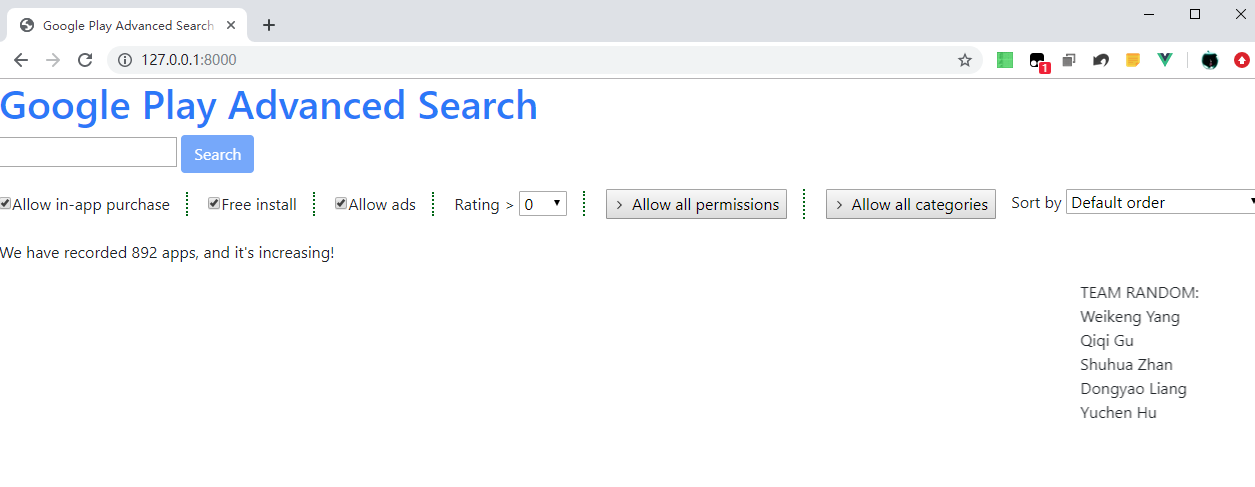
\includegraphics[width=\textwidth]{website-gray-button.png}
\caption{Initially the website has a disabled search button, but user can type something then delete them, enabling searching for empty keyword.}
\label{fig:website-gray-buton}
\end{figure}

Neither the searchApps function or the call sites verifies the length of parameter namePattern. Initially on the website, user has to type something to make the search button enabled, which might be the safe guard against searching for an empty keyword, see Figure \ref{fig:website-gray-buton}. However, if the user deletes the keyword, the search button is still enabled. Therefore user is able to search for an empty keyword, and the SQL statement doesn't limit the return rows. If there are many data in database, all data will be returned, and the execution time might be long. It can potentially become a denial of service.




Otherwise, there is a ssl verification process at Django, so I think we should do some ssl verification tests for all the ports which will send https requests to Google Play Store. As we mention that the google certificate is valid from 2020/02/12 to 2020/05/06, see Figure \ref{fig:google-certificate-information}. 

\begin{figure}[ht]
\centering
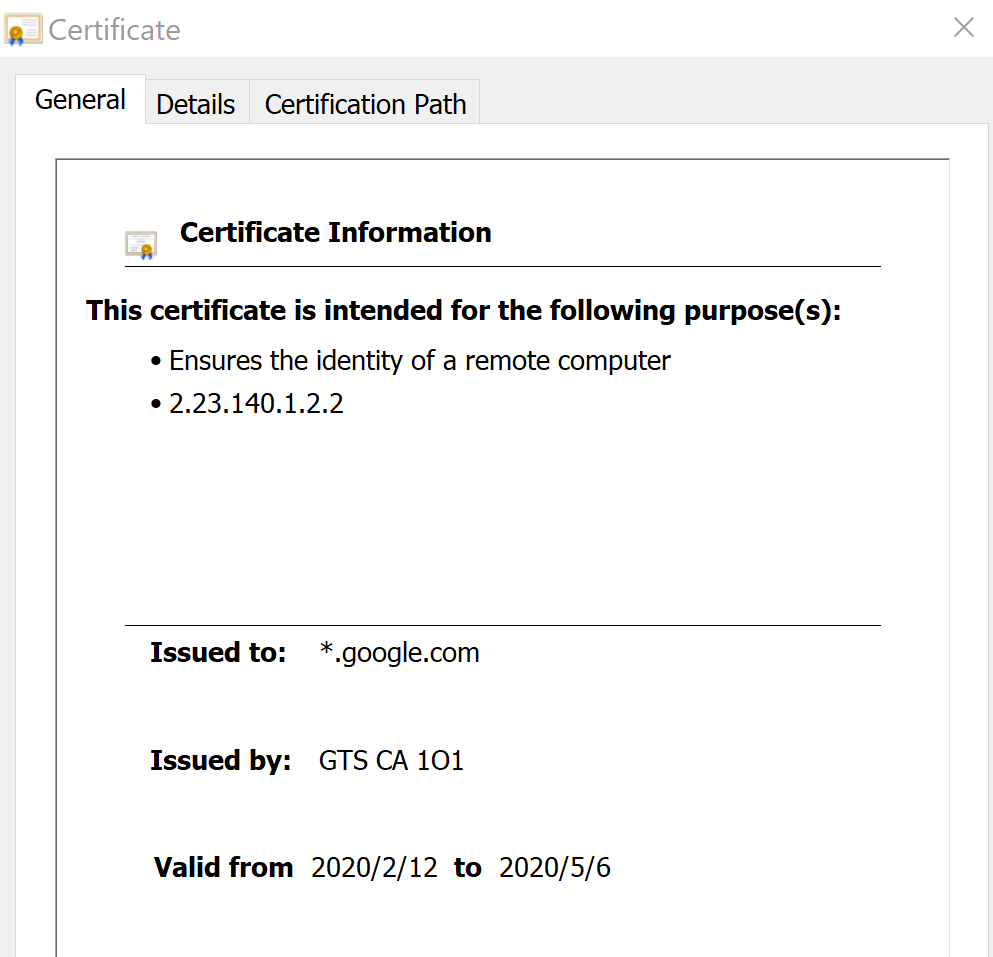
\includegraphics[width=0.7\textwidth]{google_certification_time.png}
\caption{Google Certificate Information}
\label{fig:google-certificate-information}
\end{figure}


We can change the local date time to 2020/06/18 when the google certificate expires to make sure the ssl verification is working. In listing \ref{lst:change-time}, we change local time to 2020/06/18, and run \code{src/GooglePlayAdvancedSearch/\linebreak[0]scraper/\linebreak[0]Program.py}. As expected, the scraper detects the invalid certificate, and exits.




\begin{lstlisting}[language=, frame=tb, caption=Scraper is able to reject invalid certificate, label=lst:change-time]
# date +%Y%m%d -s "20200618"
20200618
# date
Thu Jun 18 00:00:04 UTC 2020
# ./Program.py -p com.google.android.calculator
scrape these apps:
['com.google.android.calculator']
2020-06-18 00:00:13 [brickset_spider] ERROR: SSL error on https://play.google.com/store/apps/details?hl=en&id=com.google.android.calculator
Traceback (most recent call last):
  File "/anaconda3/envs/cs188/lib/python3.7/site-packages/scrapy/core/downloader/middleware.py", line 44, in process_request
    defer.returnValue((yield download_func(request=request, spider=spider)))
twisted.web._newclient.ResponseNeverReceived: [<twisted.python.failure.Failure  OpenSSL.SSL.Error: [('SSL routines', 'tls_process_server_certificate', 'certificate verify failed')]>]
\end{lstlisting}

The website module communicates with Google Play store as well. If the SSL certificate is invalid, our GooglePlayAdvancedSearch website will show some error messages to users, see Figure \ref{fig:ssl-test-on-website}. Based on the test result, we confirm the ssl verification process is working.


\begin{figure}[ht]
\centering
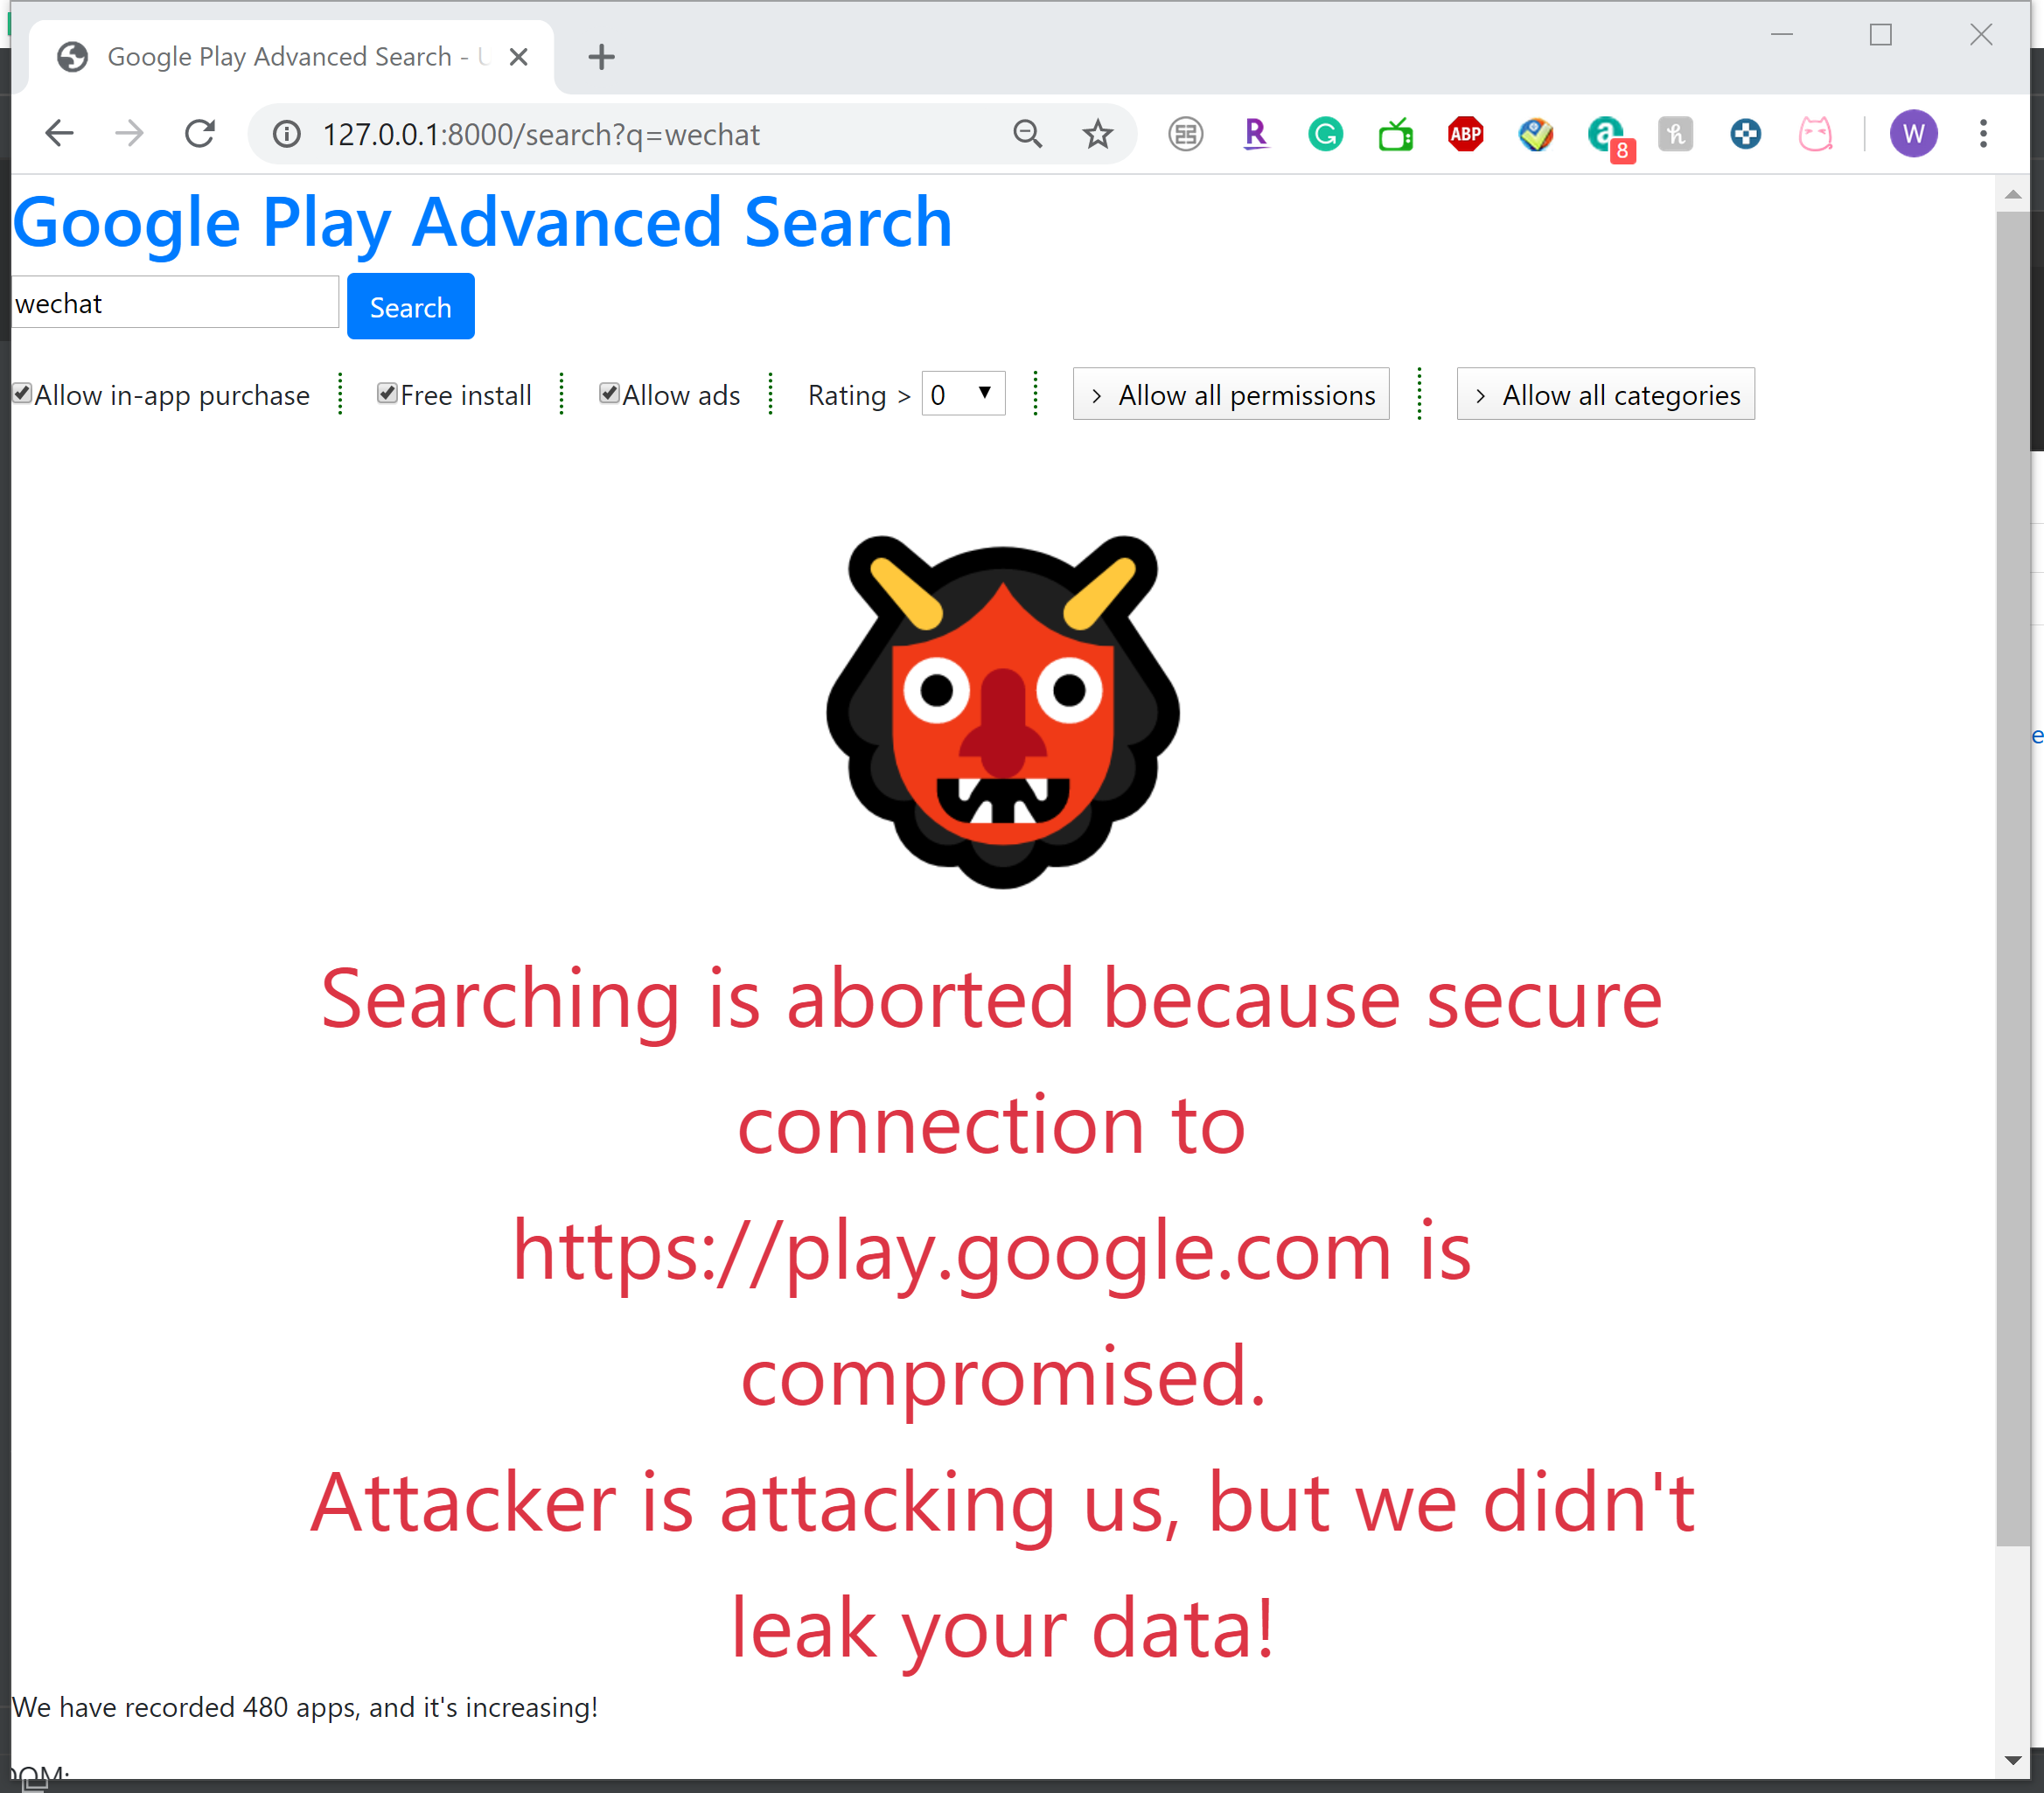
\includegraphics[width=0.7\textwidth]{ssl_test3.png}
\caption{The website module detects invalid certificates too}
\label{fig:ssl-test-on-website}
\end{figure}

% On the other hand, the scraper will also detect that the Google certificate does not meet the specifications, see figure \ref{fig:ssl-test-on-program.py}. 



% \begin{figure}[ht]
% \centering
% 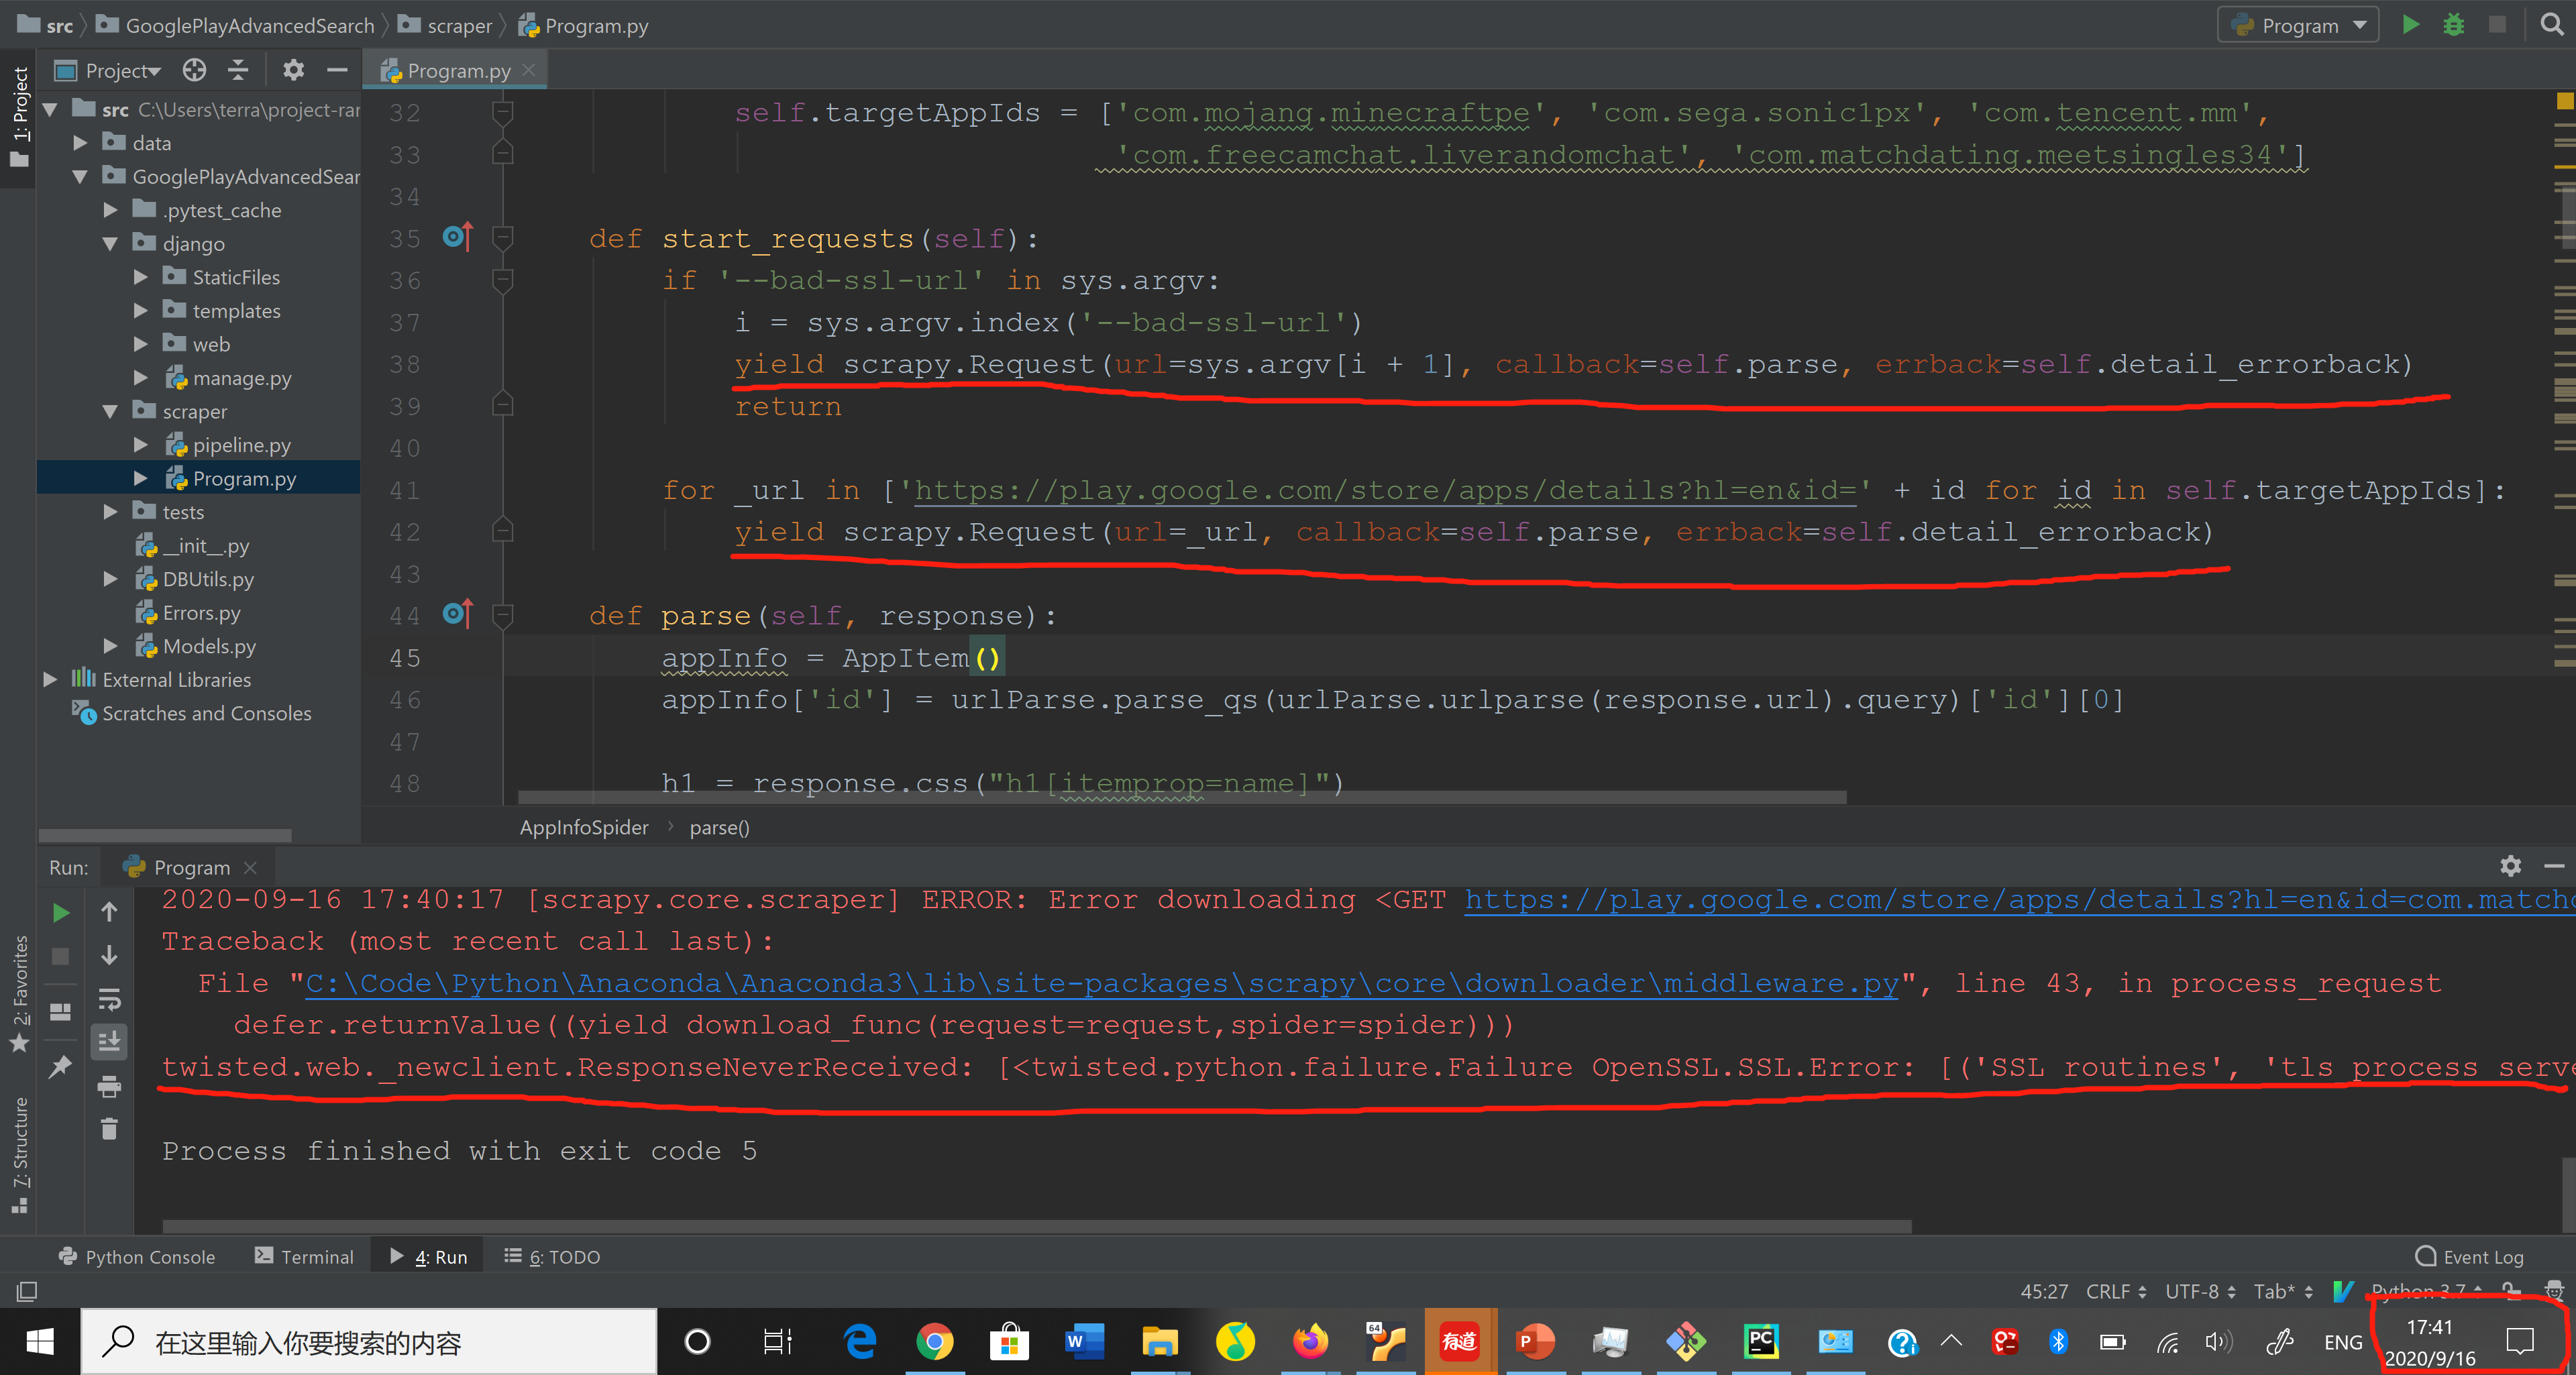
\includegraphics[width=\textwidth]{ssl_test2.png}
% \caption{ssl test on program.py}
% \label{fig:ssl-test-on-program.py}
% \end{figure}



\subsection{Automated Tests}
Project Google Play Advanced Search comes with a number of automated tests located in the tests module. These are all functional tests and the badge on the README file on the repository confirms the code passes all tests. However, there are no security tests there.

\subsection{Tool Testing Results}
\subsubsection{Nmap for Port Scanning}
We use Nmap to scan the open ports on our server. Currently we have a public ip 35.236.119.106 and domain beta.gqqnbig.me.

Running Nmap with \code{-p-} flag to scan all 65535 ports on our server.
We find ports 22, 80, 443 are open. These are exactly all ports we need to use. We didn't leave any unused port open. Detail output see Figure \ref{fig:nmap}.

\begin{figure}[ht]
\centering
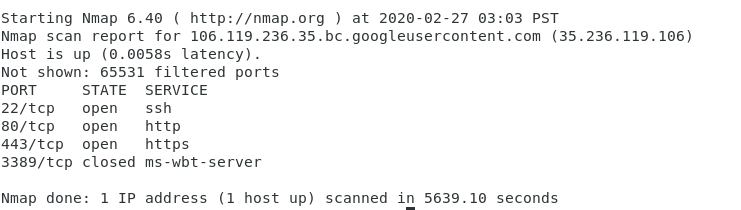
\includegraphics[width=\textwidth, frame]{nmap_log.png}
\caption{Nmap verifies only ports 22, 80, 443 are open.}
\label{fig:nmap}
\end{figure}

% \begin{center}
%     \begin{tabular}{l l l}
%         PORT & STATE & SERVICE \\
%         22/tcp & open & ssh\\
%         80/tcp & open & http\\
%         443/tcp & open & https
%     \end{tabular}
% \end{center}


\subsubsection{OWASP ZAP}
ZAP is a open source project developed by OWASP. It can help us to find the some potential security problems of our web server like SQL injection, XSS and many others.
We run zap to attack our website home page and found some Alerts:
\begin{itemize}
    \item Risk: \textcolor{orange}{low}. Cross-Domain JavaScript Source File Inclusion. We are using some third-party javascript libraries. They are:
    \begin{itemize}
        \item jQuery API:\\ \textcolor{blue}{<script src="https://code.jquery.com/jquery-3.4.1.min.js"></script>}
        \item A CDN for npm - lodash:\\ \textcolor{blue}{<script src="https://cdn.jsdelivr.net/npm/lodash@4.17.15/lodash.min.js"></script>}
        \item A progressive javascript framework - Vue.js:\\ \textcolor{blue}{<script src="https://cdn.jsdelivr.net/npm/vue@2.6.11"></script>}
    \end{itemize}
%    \item Risk: \textcolor{orange}{low}. Incomplete or No Cache-control and Pragma HTTP Header Set
%    \item Risk: \textcolor{orange}{low}. X-Content-Type-Options Header Missing on file \code{static/js/vue-click-outside.js} and \code{static/images/question.png}
    \item Risk: \textcolor{blue}{Informational}. Information Disclosure - Suspicious Comments
    \item Risk: \textcolor{blue}{Informational}. Timestamp Disclosure - Unix
\end{itemize}
One way to work around the first alert is by deploying the production mode of above third party javascript libraries to reduce the potential threat if we have more time.

Then we use ZAP to attack our search pages (eg. \url{ https://beta.gqqnbig.me/search?q=youtube&pids=33&cids=55,57}) with some permission and category filters.
And we discover more alerts (fig \ref{fig:zap-alerts}).

\begin{figure}[H]
\centering
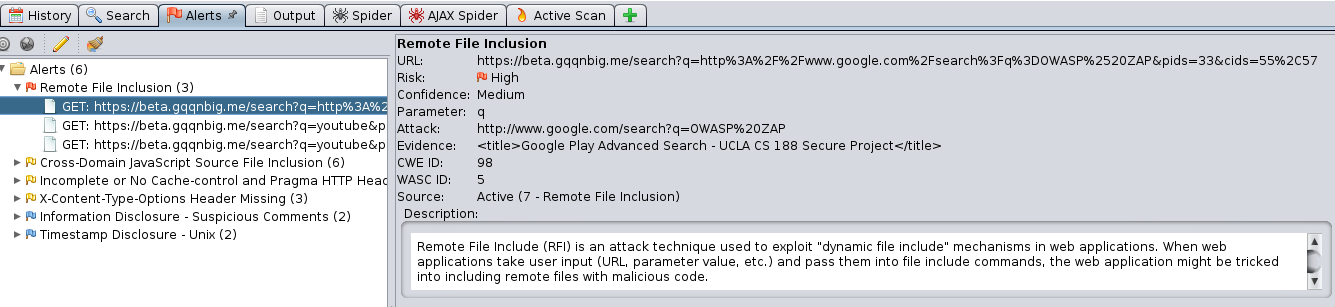
\includegraphics[width=\textwidth, frame]{zap_alerts.png}
\caption{ZAP Alerts}
\label{fig:zap-alerts}
\end{figure}

In this case, it has a \textcolor{red}{High} risk alert: \code{Remote File Inclusion}. \code{Remote File Include} (RFI) is an attack technique used to exploit "dynamic file include" mechanisms in web applications. When web applications take user input (URL, parameter value, etc.) and pass them into file include commands, the web application might be tricked into including remote files with malicious code.

ZAP suggests a solution: 
Assume all input is malicious. Use an "accept known good" input validation strategy, i.e., use a whitelist of acceptable inputs that strictly conform to specifications. Reject any input that does not strictly conform to specifications, or transform it into something that does. Do not rely exclusively on looking for malicious or malformed inputs (i.e., do not rely on a blacklist). However, blacklists can be useful for detecting potential attacks or determining which inputs are so malformed that they should be rejected outright.
When performing input validation, consider all potentially relevant properties, including length, type of input, the full range of acceptable values, missing or extra inputs, syntax, consistency across related fields, and conformance to business rules. As an example of business rule logic, "boat" may be syntactically valid because it only contains alphanumeric characters, but it is not valid if you are expecting colors such as "red" or "blue."

Looking back in our code, we do have this kind of validation. There are at most 3 elements, namely \code{q} (keyword), \code{pid} (permission id) and \code{cid} (category id). Everything else will be ignored and perform a normal search. Keyword will be passed to Google play store, pid and cid will be performing a string comparison with apps pids and cids. Looking at our code, unexpected pid and cid will be ignored since there is no such pid/cid we want to exclude. Listing \ref{lst:cp-handing} is the code snippet.


\begin{lstlisting}[frame=tb, caption=Pid/Cid Input Handling, label=lst:cp-handing]
def search(request):
	keyword = request.GET['q']
	excludedPIds = [int(n) for n in request.GET.get('pids', '').split(',') if n != '']

	excludedCIds = [int(n) for n in request.GET.get('cids', '').split(',') if n != '']

	try:
		appAccessor = AppAccessor(1)
		appInfos = appAccessor.searchApps(keyword)

		needCompleteInfo = determineAppInfoCompleteness(request)

		if needCompleteInfo:
			appInfos = getCompleteAppInfo([a['id'] for a in appInfos])

		if len(excludedPIds):
			appInfos = [a for a in appInfos if isExcluded(a['permissions'], excludedPIds) == False]
		if len(excludedCIds):
			appInfos = [a for a in appInfos if isExcluded(a['categories'], excludedCIds) == False]
    ...


def isExcluded(d: Dict, ids: List[int]):
	return any(excludedId in d for excludedId in ids)
\end{lstlisting}


\subsection{Data Security}
We attempted to use Scuba from Imperva to find the vulnerabilities in our database, but soon we realized SQLite has no concept of user accounts, and instead relies on the file system for all database permissions.

To make our database more secure, we have these following setup in our server/machine:

\begin{itemize}
    \item Only root can change the source code (usually via git pull).
    \begin{figure}[H]
    \centering
    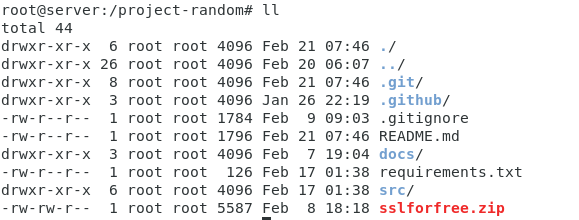
\includegraphics[width=\textwidth, frame]{sourcecodeper.png}
    \end{figure}
    \item We setup a user call ``django" whose uid is 1003 and gid is 1004. Only ``django" can write to our database (in folder \code{data}).
    \begin{figure}[H]
    \centering
    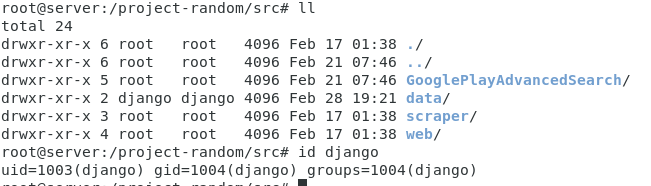
\includegraphics[width=\textwidth, frame]{databaseper.png}
    \end{figure}
    \item And run the django server using uwsgi with uid 1003 and gid 1004: \code{nohup uwsgi --uid 1003 --gid 1004 --socket \linebreak[4] /tmp/GooglePlayAdvancedSearch.sock --module web.wsgi \linebreak[4] --chmod-socket=666 \&> /tmp/django.log \&}
\end{itemize}

\subsection{DDOS attack}
We wrote a simple python script (fig \ref{fig:ddos}) to send 20 requests to our server. In the result (fig \ref{fig:ddos-out}), only some requests have \code{staus\_code}=200, others are 503 because we configure a rate limit 10 access per second in Nginx. 

The rate limit can't be too low because we do use AJAX to access some APIs.

This (fig \ref{fig:503}) is how it looks like in the browser when we refresh our page more than once per second.



\begin{figure}[ht]
\centering
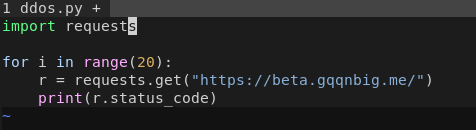
\includegraphics[width=0.8\textwidth]{ddos.png}
\caption{send 20 requests to server}
\label{fig:ddos}
\end{figure}

\begin{figure}[ht]
\centering
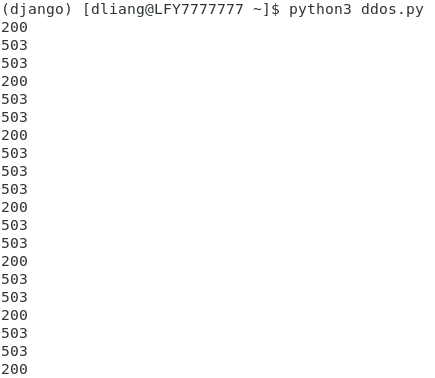
\includegraphics[width=0.7\textwidth]{ddos-out.png}
\caption{Status Codes from 10 Requests}
\label{fig:ddos-out}
\end{figure}

\begin{figure}[ht]
\centering
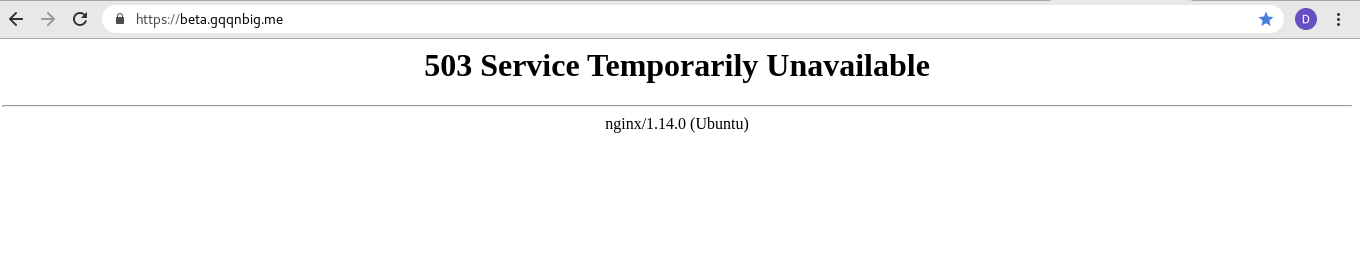
\includegraphics[width=\textwidth]{503.png}
\caption{503 Response}
\label{fig:503}
\end{figure}

\subsection{SSL Test}
We also use an online tool \code{immuniweb} to perform a ssl security check. See Figure \ref{fig:immuniweb}. The full result is available on \url{https://www.immuniweb.com/ssl/?id=TWn6BgrW} Although we have a good overall score, we still have some issue:

\begin{itemize}
    \item Not providing an intermediate certificate.
    \item Not providing OCSP Stapling.
    \item Some default ciphers from TSL 1.1 and 1.2 are non-compliant with HIPAA guidance.
    \item Our server doesn't enforce HTTP Strict Transport Security(HSTS)
\end{itemize}

We don't have an intermediate certificate because the SSL certificate is free. We don't configure HSTS because the free SSL certificate expires in 3 months. We have to renew it very often. It's possible that when we are changing the certificate, our patrons come to the website. If HSTS is enabled, they will be blocked from visiting our site by their browser. 

For other two issues, we believe it's good to implement them on the server.


\begin{figure}[ht]
\centering
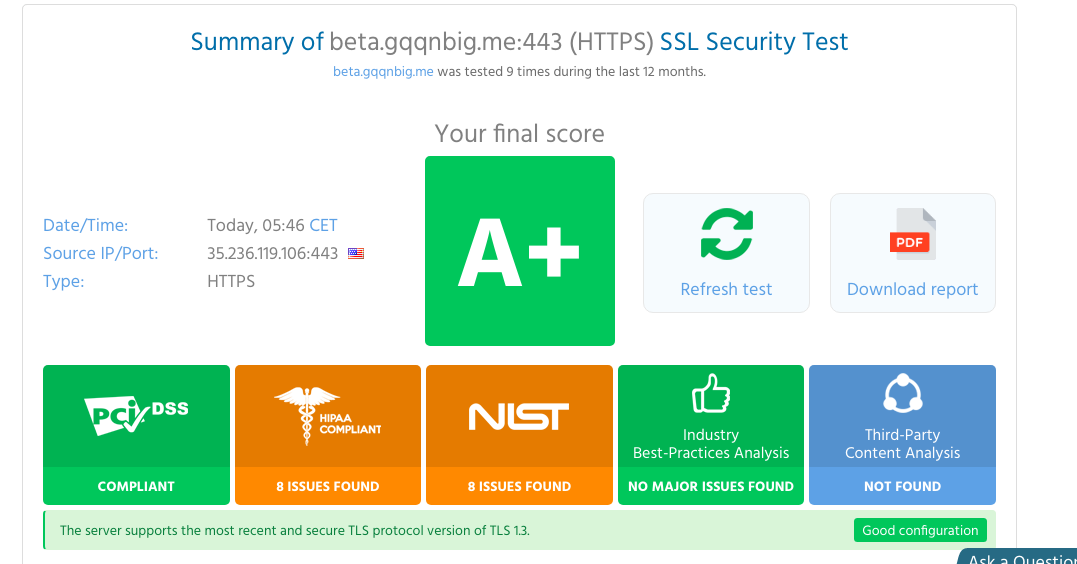
\includegraphics[width=0.7\textwidth]{immuniweb.png}
\caption{immuniweb.com gives A+ score on the server}
\label{fig:immuniweb}
\end{figure}





\section{Recommendations for future evaluations}

%Requirement: If time and resources did not permit you to study the system as fully as you feel was desirable, you should discuss how future efforts to better understand the security of the system should be directed. You should also discuss conditions under which a fresh review might be required, such as the addition of obvious major extensions to the prototype of the project. 

%Code review: Perform flow analysis carefully within functions you examine

First, we review our initial project design document. We don't implement all the functions of our GooglePlayAdvancedSearch website. For example, it should allow users search the apps depend on the rating area or no advertising. If we have enough time, we will implement all the functions we mentioned in the design document or increase some advanced features. We may need to think more comprehensively about software security.

Secondary, during our security test process, we find that the database we choose was not good enough in terms of security. Some test tool shows that SQLite doesn't do much to keep our data private or secure, or even to set up a password to verify that our visitors qualify. If we have more time, we will choose a more secure database, like MySQL.

Other Python 3.7 vulnerabilities are not immediately relevant to our project because we are not using the affected functions. We should check if the dependencies are using them, but due to time constraint, we didn't do.

Although we tested that our code evaluates Google's ssl certificate by changing local time to make it outdated, we can still do a man-in-the-middle attack by spoofing our server. 

\section{Lessons learned by performing the security evaluation}
\subsection{When designing the system}
When designing a software, we should always think of potential security issues beforehand by performing risks analysis. With the tools and principles we have learned in class, one can always get a general idea of the problems that a project might be facing. The secure design principles suggest that we follow an economy of mechanism, have fail-safe defaults, complete mediation, least privilege, psychological acceptability, compromise recording, defense in depth, design for updating, open design, promote privacy and be reluctant to trust. The most fundamental part of our team's understanding is that one should not do extra work on what we don’t need and grant least amount of access as Economy of mechanism and fail-safe defaults suggest. We should default to lack of access. It’s convenient to grant all access without really considering their functiok/nalities individually but it’s very dangerous to do so since malicious hackers can easily attack the product by installing and executing malicious scripts. Forgetting to grant access may cause errors but it keeps the software secure. Similar reasons for granting least privilege, a secure system should give the minimum access and permissions. For example, since our web server interacts with a database, we don’t want the server to have full access of the database in case the server is hacked and we also don’t want users to have access to gain information from database for privacy concerns. For now our database does not store any type of personal information so we should be safe from that but in case we have account access for users, we should always think of this issue beforehand. Also when designing a product, it’s essential to find a balance between security and a better user experience. The key point is that we want our website to be convenient for users and making it too complicated would lead to the loss of customers.
\subsection{While Secure Coding}
While coding, we should think of major problems areas for security purposes. It’s important to keep in mind these problems in mind and scan through the major problem areas during the development of the system. For example, since we ask users for keyword inputs for searching, we were thinking if we would have buffer overflow attack when users inputs are too long. However, as we did some research we found out that the latest version of the 3.3.4 python is safe from buffer overflow with the vulnerability has been patched.
\subsection{When Evaluating the Security of the System}
After going through the above process and when it comes to evaluating, we are able to narrow down the scope to specific problem areas based on individual types of the design since different types of projects may have different kinds of security issues. For example, our project does not have problems with encryption and decryption but we have problems such as SQL injections since we ask users for input keywords. Therefore, for efficient evaluating, we should focus more on the higher potential problems regarding on database. However, we always need to keep an eye on the general problems like error handling and checking return codes since all programs have a potential risks of making mistakes on these areas. When testing the system, it's also useful to consider edge cases like running on an unprivileged mode and check if it can do work on higher privilege mode. In addition, it's helpful to create a list of a structure of the code to check if it creates any potential bugs such as problems caused by race conditions. Sometimes looking all the problems on our own is not enough and testing tools can be a great help too.

\section{Work breakdown}
Qiqi Gu - He is responsible for External Components Evaluation and part of Code Review. He found keyword denial of service issue and proofread the report.

Dongyao Liang - responsible to use tools to test our security and evaluate our server.

Shuhua Zhan - responsible for lessons learned section of the report and participated in code review. 

Yingze Hu - responsible for security design review.

Weikeng Yang - responsible for Interactive application security testing (IAST)




\begin{thebibliography}{99}
    \bibitem{django-security-issues} \citeWeb{Archive of security issues}{https://docs.djangoproject.com/en/3.0/releases/security/}{2020-02-25}
    \bibitem{scrapy-s3} \citeWeb{S3FilesStore can use a lot of memory}{https://github.com/scrapy/scrapy/issues/482}{2020-02-25}
    \bibitem{pyjson5} \citeWeb{pyjson5: A Python implementation of the JSON5 data format
}{https://github.com/dpranke/pyjson5}{2020-02-25}
    \bibitem{double-free} \citeWeb{Doubly freeing memory}{https://owasp.org/www-community/vulnerabilities/Doubly_freeing_memory}{2020-02-25}
    \bibitem{requests-security-vulnerabilities} \citeWeb{Vulnerability Disclosure}{https://requests.readthedocs.io/en/master/community/vulnerabilities/}{2020-02-25}
    \bibitem{scrapy-xml} \citeWeb{Fixed XXE flaw in sitemap reader}{https://github.com/scrapy/scrapy/pull/676}{2020-02-25}
    \bibitem{snyk-twisted} \citeWeb{twisted vulnerabilities}{https://snyk.io/vuln/pip:twisted}{2020-02-25}
    \bibitem{cve-twisted} \citeWeb{Twisted Vulnerability Statistics}{https://www.cvedetails.com/product/55543/Twistedmatrix-Twisted.html?vendor_id=16756}{2020-02-25}
    \bibitem{windows7} \citeWeb{Windows 7 support ended on January 14, 2020}{https://support.microsoft.com/en-us/help/4057281/windows-7-support-ended-on-january-14-2020}{2020-02-26}
    \bibitem{python37-vulnerability} \citeWeb{Security vulnerabilities - Python Security Vulnerabilities}{https://python-security.readthedocs.io/vulnerabilities.html}{2020-02-26}
    \bibitem{bpo-30458} \citeWeb{[security][CVE-2019-9740][CVE-2019-9947] HTTP Header Injection (follow-up of CVE-2016-5699)}{https://bugs.python.org/issue30458}{2020-02-26}
    \bibitem{bpo-30730} \citeWeb{[security] Injecting environment variable in subprocess on Windows}{https://bugs.python.org/issue30730}{2020-02-26}
    \bibitem{CVE-2019-9636} \citeWeb{CVE-2019-9636}{https://linux.oracle.com/cve/CVE-2019-9636.html}{2020-02-26}
    \bibitem{jquery-341} \citeWeb{jquery@3.4.1 vulnerabilities}{https://snyk.io/vuln/npm:jquery@3.4.1}{2020-02-28}
    \bibitem{html-standard-script} \citeWeb{HTML
Living Standard}{https://html.spec.whatwg.org/multipage/scripting.html\#the-script-element}{2020-02-28}
\end{thebibliography}

%\section{Supplementary materials}
%Requirement: If your analysis produced useful artifacts (such as automated reports, screen shots demonstrating problems, scripts used to test functionality, etc.), include these in appendices, where possible. For things that are not easily embedded in a 
%report (such as a video demonstrating how to exploit a security flaw), upload them as separate files when you submit the report. You can also provide links to supplementary materials, but if you do, make sure that the materials are in a location that can be accessed by others, not in a private area. Make sure that your supplementary material section indicates which files are uploaded as part of your report, which links are associated with your report, and what each file or link represents.  
% 

\end{document}